\documentclass[tikz,border=5pt]{standalone}
\usepackage{tikz}
\usepackage{xcolor}
\usepackage{amsmath}
\usepackage{amssymb}

\usetikzlibrary{shapes.geometric}
\usetikzlibrary{decorations.pathmorphing}
\usetikzlibrary{positioning}
\usetikzlibrary{shadows}
\usetikzlibrary{calc}

\definecolor{quantumblue}{RGB}{50,150,255}
\definecolor{quantumgreen}{RGB}{100,255,150}
\definecolor{quantumpurple}{RGB}{150,100,255}
\definecolor{quantumorange}{RGB}{255,150,50}
\definecolor{consensuscolor}{RGB}{200,50,200}
\definecolor{superpositioncolor}{RGB}{100,200,255}

\begin{document}
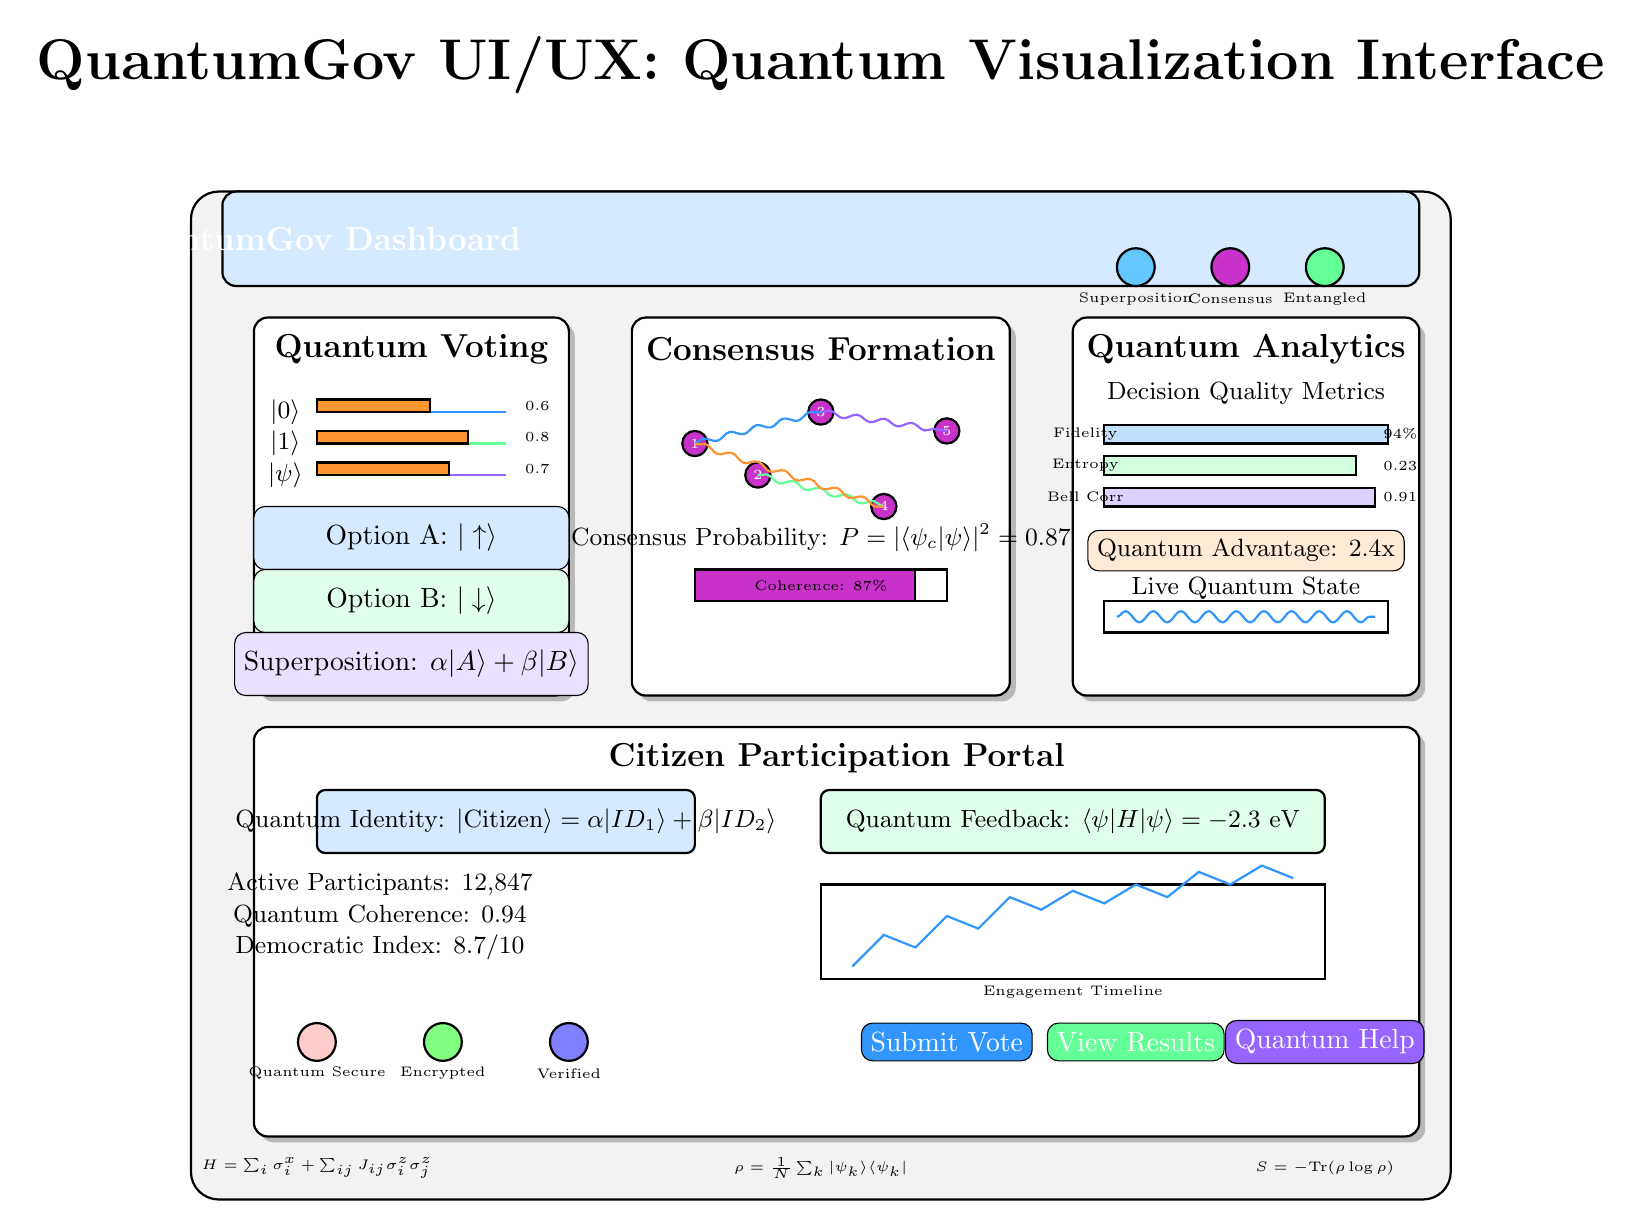
\begin{tikzpicture}[scale=0.8]

% Title
\node[font=\huge\bfseries] at (10,18) {QuantumGov UI/UX: Quantum Visualization Interface};

% Main Dashboard Container
\draw[thick, rounded corners=10pt, fill=gray!10] (0,0) rectangle (20,16);

% Header Bar with Quantum State Indicators
\draw[thick, rounded corners=5pt, fill=quantumblue!20] (0.5,14.5) rectangle (19.5,16);
\node[font=\large\bfseries, white] at (2,15.2) {QuantumGov Dashboard};

% Quantum State Indicators
\draw[thick, fill=superpositioncolor] (15,14.8) circle (0.3);
\node[font=\tiny] at (15,14.3) {Superposition};

\draw[thick, fill=consensuscolor] (16.5,14.8) circle (0.3);
\node[font=\tiny] at (16.5,14.3) {Consensus};

\draw[thick, fill=quantumgreen] (18,14.8) circle (0.3);
\node[font=\tiny] at (18,14.3) {Entangled};

% Left Panel: Quantum Voting Interface
\draw[thick, rounded corners=5pt, fill=white, drop shadow] (1,8) rectangle (6,14);
\node[font=\large\bfseries] at (3.5,13.5) {Quantum Voting};

% Quantum State Visualization
\draw[thick, quantumblue] (2,12.5) -- (5,12.5);
\draw[thick, quantumgreen] (2,12) -- (5,12);
\draw[thick, quantumpurple] (2,11.5) -- (5,11.5);

\node[font=\small] at (1.5,12.5) {$|0\rangle$};
\node[font=\small] at (1.5,12) {$|1\rangle$};
\node[font=\small] at (1.5,11.5) {$|\psi\rangle$};

% Probability Amplitudes
\foreach \y/\val in {12.5/0.6, 12/0.8, 11.5/0.7} {
    \draw[thick, fill=quantumorange] (2,\y) rectangle (2+\val*3,\y+0.2);
    \node[font=\tiny] at (5.5,\y+0.1) {\val};
}

% Vote Options with Quantum States
\node[draw, rounded corners, fill=quantumblue!20, minimum width=4cm, minimum height=0.8cm] at (3.5,10.5) {Option A: $|\uparrow\rangle$};
\node[draw, rounded corners, fill=quantumgreen!20, minimum width=4cm, minimum height=0.8cm] at (3.5,9.5) {Option B: $|\downarrow\rangle$};
\node[draw, rounded corners, fill=quantumpurple!20, minimum width=4cm, minimum height=0.8cm] at (3.5,8.5) {Superposition: $\alpha|A\rangle + \beta|B\rangle$};

% Center Panel: Consensus Visualization
\draw[thick, rounded corners=5pt, fill=white, drop shadow] (7,8) rectangle (13,14);
\node[font=\large\bfseries] at (10,13.5) {Consensus Formation};

% Quantum Consensus Network
\foreach \i/\x/\y in {1/8/12, 2/9/11.5, 3/10/12.5, 4/11/11, 5/12/12.2} {
    \draw[thick, fill=consensuscolor] (\x,\y) circle (0.2);
    \node[font=\tiny, white] at (\x,\y) {\i};
}

% Entanglement Lines
\draw[thick, quantumblue, decorate, decoration={snake,amplitude=1pt}] (8,12) -- (10,12.5);
\draw[thick, quantumgreen, decorate, decoration={snake,amplitude=1pt}] (9,11.5) -- (11,11);
\draw[thick, quantumpurple, decorate, decoration={snake,amplitude=1pt}] (10,12.5) -- (12,12.2);
\draw[thick, quantumorange, decorate, decoration={snake,amplitude=1pt}] (11,11) -- (8,12);

% Consensus Probability
\node[font=\small] at (10,10.5) {Consensus Probability: $P = |\langle\psi_c|\psi\rangle|^2 = 0.87$};

% Quantum Coherence Meter
\draw[thick] (8,9.5) rectangle (12,10);
\draw[thick, fill=consensuscolor] (8,9.5) rectangle (11.5,10);
\node[font=\tiny] at (10,9.75) {Coherence: 87\%};

% Right Panel: Decision Analytics
\draw[thick, rounded corners=5pt, fill=white, drop shadow] (14,8) rectangle (19.5,14);
\node[font=\large\bfseries] at (16.75,13.5) {Quantum Analytics};

% Decision Quality Metrics
\node[font=\small] at (16.75,12.8) {Decision Quality Metrics};

% Quantum Fidelity
\draw[thick, fill=quantumblue!30] (14.5,12) rectangle (19,12.3);
\node[font=\tiny] at (14.2,12.15) {Fidelity};
\node[font=\tiny] at (19.2,12.15) {94\%};

% Entanglement Entropy
\draw[thick, fill=quantumgreen!30] (14.5,11.5) rectangle (18.5,11.8);
\node[font=\tiny] at (14.2,11.65) {Entropy};
\node[font=\tiny] at (19.2,11.65) {0.23};

% Bell State Correlation
\draw[thick, fill=quantumpurple!30] (14.5,11) rectangle (18.8,11.3);
\node[font=\tiny] at (14.2,11.15) {Bell Corr};
\node[font=\tiny] at (19.2,11.15) {0.91};

% Quantum Advantage Score
\node[draw, rounded corners, fill=quantumorange!20, font=\small] at (16.75,10.3) {Quantum Advantage: 2.4x};

% Real-time Quantum State Monitor
\node[font=\small] at (16.75,9.7) {Live Quantum State};
\draw[thick] (14.5,9) rectangle (19,9.5);
\draw[thick, quantumblue, decorate, decoration={snake,amplitude=2pt}] (14.7,9.25) -- (18.8,9.25);

% Bottom Panel: Citizen Participation Interface
\draw[thick, rounded corners=5pt, fill=white, drop shadow] (1,1) rectangle (19.5,7.5);
\node[font=\large\bfseries] at (10.25,7) {Citizen Participation Portal};

% Quantum Identity Verification
\draw[thick, rounded corners=3pt, fill=quantumblue!20] (2,5.5) rectangle (8,6.5);
\node[font=\small] at (5,6) {Quantum Identity: $|\text{Citizen}\rangle = \alpha|ID_1\rangle + \beta|ID_2\rangle$};

% Participation Metrics
\node[font=\small] at (3,5) {Active Participants: 12,847};
\node[font=\small] at (3,4.5) {Quantum Coherence: 0.94};
\node[font=\small] at (3,4) {Democratic Index: 8.7/10};

% Quantum Feedback Loop
\draw[thick, rounded corners=3pt, fill=quantumgreen!20] (10,5.5) rectangle (18,6.5);
\node[font=\small] at (14,6) {Quantum Feedback: $\langle\psi|H|\psi\rangle = -2.3$ eV};

% Real-time Engagement Graph
\draw[thick] (10,3.5) rectangle (18,5);
\draw[thick, quantumblue] (10.5,3.7) -- (11,4.2) -- (11.5,4) -- (12,4.5) -- (12.5,4.3) -- (13,4.8) -- (13.5,4.6) -- (14,4.9) -- (14.5,4.7) -- (15,5) -- (15.5,4.8) -- (16,5.2) -- (16.5,5) -- (17,5.3) -- (17.5,5.1);
\node[font=\tiny] at (14,3.3) {Engagement Timeline};

% Quantum Security Indicators
\draw[thick, fill=red!20] (2,2.5) circle (0.3);
\node[font=\tiny] at (2,2) {Quantum Secure};

\draw[thick, fill=green!50] (4,2.5) circle (0.3);
\node[font=\tiny] at (4,2) {Encrypted};

\draw[thick, fill=blue!50] (6,2.5) circle (0.3);
\node[font=\tiny] at (6,2) {Verified};

% Quantum Buttons and Controls
\node[draw, rounded corners, fill=quantumblue, text=white, minimum width=2cm] at (12,2.5) {Submit Vote};
\node[draw, rounded corners, fill=quantumgreen, text=white, minimum width=2cm] at (15,2.5) {View Results};
\node[draw, rounded corners, fill=quantumpurple, text=white, minimum width=2cm] at (18,2.5) {Quantum Help};

% Mathematical Annotations
\node[font=\tiny] at (2,0.5) {$H = \sum_i \sigma_i^x + \sum_{ij} J_{ij}\sigma_i^z\sigma_j^z$};
\node[font=\tiny] at (10,0.5) {$\rho = \frac{1}{N}\sum_k |\psi_k\rangle\langle\psi_k|$};
\node[font=\tiny] at (18,0.5) {$S = -\text{Tr}(\rho\log\rho)$};

\end{tikzpicture}
\end{document}